\documentclass[12pt]{article}
\usepackage{hyperref, graphicx, float} 
\graphicspath{{./pics/}}
% Title Page
\title{FEEG6003: Advanced Computation Methods II - OpenMp Coursework}
\author{Marian Daogaru, 25685252}

\date{17/04/2017}

\usepackage{geometry}
\geometry{a4paper,
	total={170mm,257mm},
	left=25mm, right=25mm,
	top=25mm, bottom=25mm,
}

\usepackage{fancyhdr}
\pagestyle{fancy}
\fancyhf{}
\rhead{M. Daogaru, 25685252}
\lhead{FEEG6003}
\renewcommand{\footrulewidth}{0.9pt}
\cfoot{\thepage}

\begin{document}
	\maketitle
	
	\pagebreak
	\section{Introduction}
	In this report, the different methods of using OpenMP parallelisation shall be presented. As a benchmark of complexity, two different functions (loop1 and loop2) shall be used. 
	
	In the first part, the different standard OpenMp methods of parallelisation will be presented for both loops. These scheduling methods are:
		\begin{enumerate}
			\item static 
			\item auto
			\item static with chunksize n
			\item dynamic with chunksize n
			\item guided with chunksize n
		\end{enumerate}
	
	In the second half, a new method of parallelisation is created and compared with the schedule that executed each function in the least amount of time.
	
	In this exercise, each loop is executed 100 times in order to determine its execution time. Running each only one time would produce quite biased results, as the CPU might be somewhat more used at that particular point than normal, thus slowing the execution time. While executing the loops many times, this will produce an averaged effect. However, the execution time recorded, and thus the time presented throughout this report, is the time took to execute the 100 repetitions. This does not provide an indication of each repetition, just an average. In addition, as the time took to execute one single function is quite short (as shall be presented later), 100 reps might not be enough to get a true average of the execution, but it is sufficient for the scope of this report.
	
	Both loops follow a similar execution patters. They both compute a value based on a different variable. The calculation is inside a 2 layer nested for loop, with the first layer iterating from 0 to N (N is pre-set to 729 in this exercise), while the second layer being different for each function. In the first function, the value computed is the cosine of the variable. In the second function, the computed value is more complicated. 
	
	The scope of this exercise is to parallelise the outer loop in each function, without influencing the inner loops. For this report, the code produced was executed on the ARCHER supercomputer.

	\pagebreak
	
	\section{Static, Dynamic and Guided implementation}
	
	For this exercise, both function were required to be parallelised using the above mentioned scheduling options. In order to do so, new functions were created using the respective scheduling. Parallelisation was relatively straightforward. As the initial code was in C, the remaining code was also created in C. As such, the command \textbf{\#pragma omp parallel}. 
	
	Having this set up in the main part of the code, the remaining part was created as follows. The sections which did not include the execution of 100 repetitions were executed only by the main thread. However, the parts where parallelisation was required, this barrier was lifted, enabling all threads to operated. In addition, as each thread was executing the loops at different speeds, once finished, they would wait the remaining threads to finish, before moving to the single threads operation zone.
	
	As required, each function was initially run with the 5 different schedules using 6 threads. In addition, the chunk size for the \textit{static, dynamic and guided} was set for the following values: 1, 2, 4, 8, 16, 32, and 64. 
	
	\subsection{Loop1}
	\begin{figure}[H]	
		\centering
		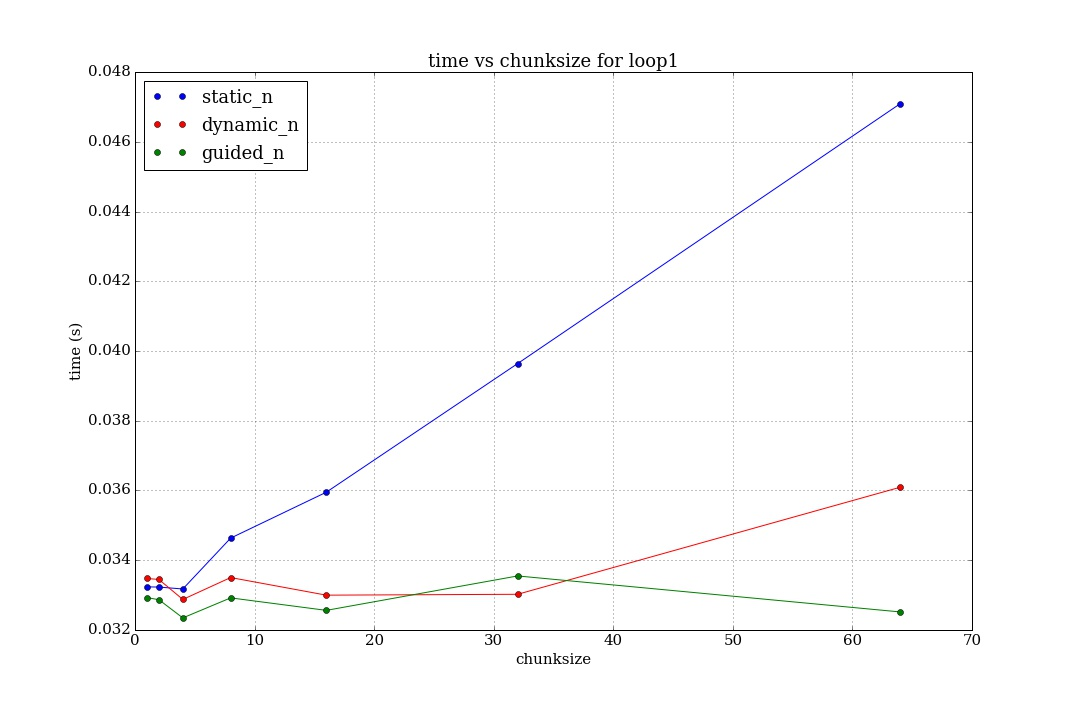
\includegraphics[scale=0.4]{loop1.jpeg}
		\caption{Execution time for different chunk sizes for loop1.}\label{loop1}
	\end{figure}
	
	Figure \ref{loop1} presents the execution time for the 3 different scheduling options, for the different chunk sizes. It can be seen that the static scheduling with different chunk size creates an increase in execution time, while te dynamic and guided are roughly the same for the majority of the chunk sizes. As the purpose is to obtain the scheduling that provides the least execution time, Guided with chunk size 4 would seem the best options. However, the two other remaining scheduling options remaining provide a better time. The simple Static averages at 0.01477s, while the Auto is just over at 0.014805s. Consequently, the simple static schedule was chosen as the optimum for loop1.
	
	This was an expected result, as loop1 is a relatively simple algorithm, and the overhead created by the more complicated schedules is not compensating for the speed-up the create. 
	
	\subsection{Loop2}
	\begin{figure}[H]	
		\centering
		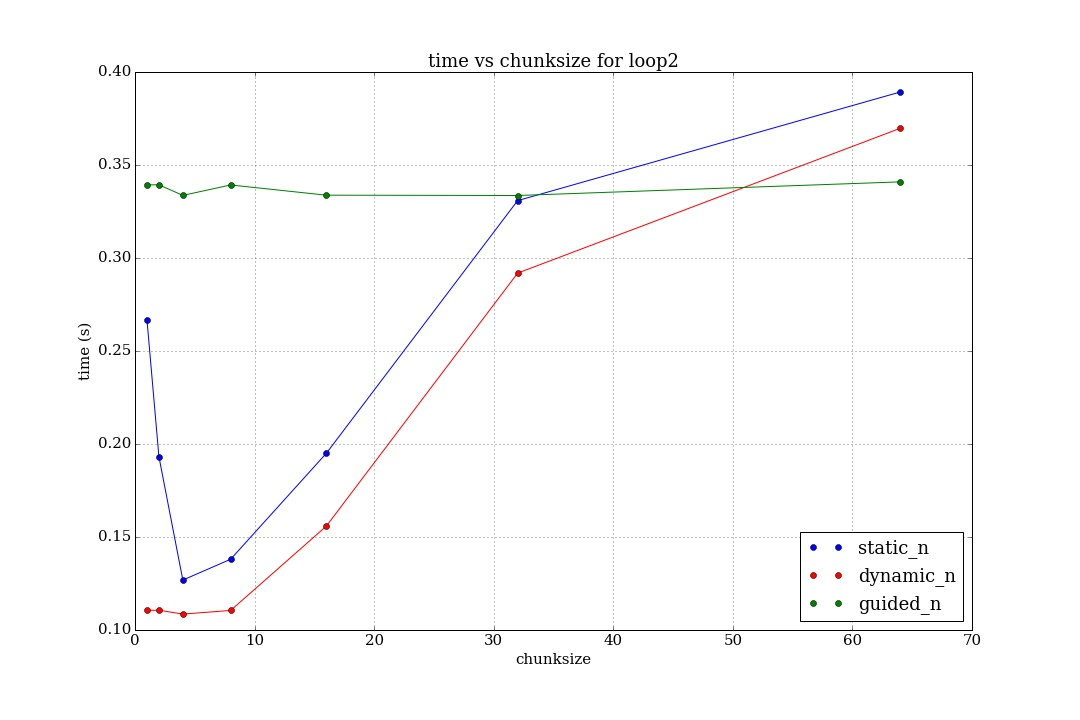
\includegraphics[scale=0.4]{loop2.jpeg}
		\caption{Execution time for different chunk sizes for loop2.}\label{loop2}
	\end{figure}

	Figure \ref{loop2} presents the execution times the 3 schedules, using the above mentioned chunk sizes. It can be observed that Dynamic with chunk size of 4 presents the best execution time between all. In addition, it is also faster that the simple static and auto scheduling, each with an execution time of around 0.405s.
	
	Two interesting behaviours can be observed in this graph. Firstly, the Static schedule with different chunk sizes initially decreases in execution time while the chunk size increases, but then it goes back up. Secondly, the dynamic schedule follows a similar pattern, but the decrease in execution time is less dramatic. These behaviours are again explained by the overhead created by the different schedules not compensating for the speed up.
	
	As this function is more complicated, the results are expected, with more complicated schedules to provide a better time than the simpler ones. As such, for \textit{loop2}, Dynamic scheduling with chunk size 4 was chosen as the best parallelisation schedule. 
	
	\pagebreak
	
	
	\section{Speed-up choice and implementation}
	As discussed before, for the first loop, the simple static scheduling provided the least executing time. For the second loop2, the Dynamic schedule, with chunk size of 4, was concluded to provide the best performance. In this chapter, these two scheduling options for parallelisation were investigated for a different number of threads, to observe the speed up. As such, the execution time of 100 repetitions of executing each function, was measure for using 1, 2, 3, 6, 12, and 24 threads.
	
	\begin{figure}[H]	
		\centering
		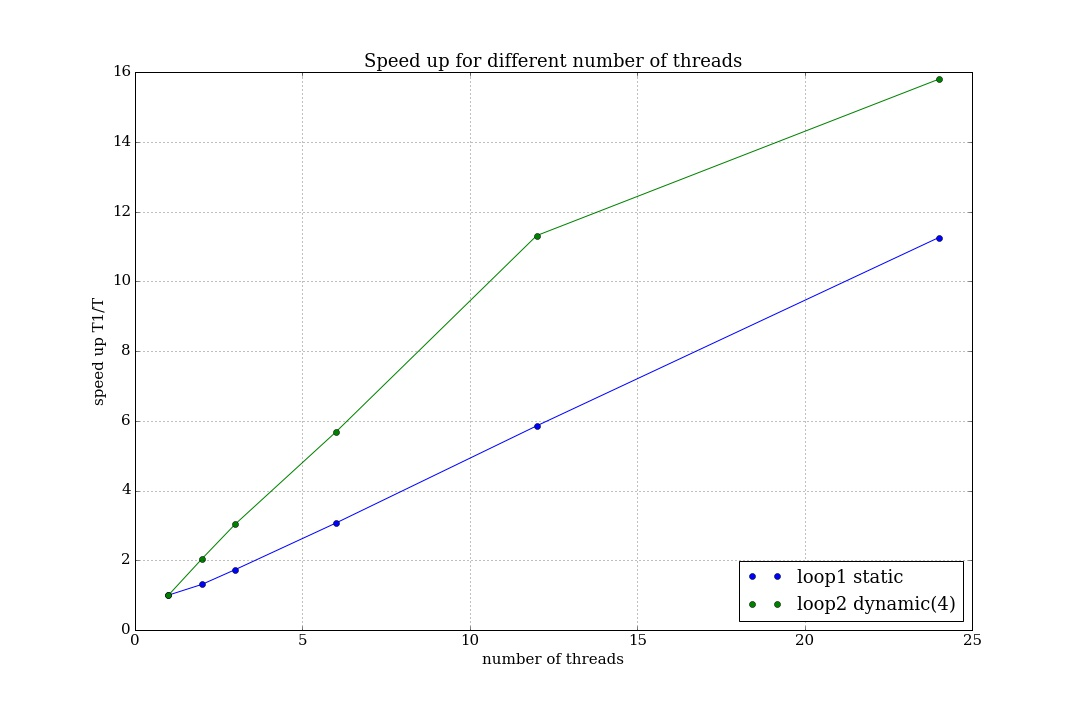
\includegraphics[scale=0.4]{speed_up.jpeg}
		\caption{Relative execution time for both function for different number of threads.}\label{up}
	\end{figure}	

	Figure \ref{up} presents the speed up provided by using an increasing number of threads. The speed up values are defined as the execution time using only one threads divided by the execution time using the given the current number of threads. It can be clearly observed that the speed up is linear for both functions. For loop2, there is a different gradient between the last 2 points. This is caused by complexity of the function and the overhead. 
	
	The linear pattern observed is appropriate for this experiment. While the number of threads is increased, the execution time should go down. While increasing the number of threads present might make improve the results, at some point, the overhead created will be more detrimental. In addition, given the fact that the repetitions number is quite low (100), this might affect how the overall overhead created might should affect the results. 
	
	\pagebreak
	
	\section{Affinity implementation}
	\subsection{Local set creation}
	The initial implementation of the (new) affinity scheduling is represented by the data distribution between threads. In the first part of this report, the default schedules would autonomously split the iterations they were required to solve in the for loops. However, for this case, this must be done by the code.
	
	Firstly, the current number of initialised threads is stored (\textit{p}). Next, each thread is assigned an equal number of N/p. If p does not divide N, then a number of threads equal to the remainder, starting from the first thread, are allocated an addition iteration. This way, we have a relatively even distribution of workload between the threads. This is called \textit{the local set}.
	For each thread, the values of the start and the end of the local set are stored. An array (\textit{start\_loc}) stores the starting position of each thread, while an array (\textit{stop\_loc}) stores the position of the end of each thread. The stop location of the i-1 thread is the start location of the ith thread.
	
	Next, each thread starts to execute a chunk from their local set equal to $local\_set/p$. If the p does not divide the local set, the chunk takes the value of the smallest integer bigger than the value given by the division. This way, it is ensured that the next steps will function properly, and each thread will actually finish their local set. 
	
	After the thread has executed the current chunk, it subtracts the chunk from its local set. It then repeats the previous step until the local set is finished. As an example: consider that we have N=101 (iterations) and 5 threads running. Thus, each thread will have an initial local set of 20 (100/5), except for the first thread which will have 21 iterations. Next, the last 4 threads will execute 4 iterations from their local set (20/5), while the first thread will execute 5 iterations (21/5=4.2, thus 5 being the next integer). Not each local set will become 16 (20-4 and 21-5). Now, each thread will execute 4 iterations (16/5=3.2, thus 4 being the next integer). The process will repeat until each local set reaches its end.
	
	
	\subsection{Parallelisation}
	Once parallelisation, several important aspects of this problem change. Firstly, each thread will prioritise its own local set, following the execution pattern described earlier. 
	
	Once a thread has finished its finished its iterations, it will start to help other threads. The important aspect is choosing the appropriate thread. The priority is set to selecting the thread which has the most iterations left in its local set. Once the appropriate thread has been chosen, while it continues to execute its current chunk, the free thread will create a new chunk of size equal to the remaining local set divide by the number of operating threads, as described in the previous section. 
	
	The problem with this implementation arises when selecting the most loaded threads. If left unrestricted, the behaviour will default the several free threads and the most loaded thread to all execute the same chunk, rather the consecutive chunks. This represents a considerable problem. However, the solution to this implementation is restricting the creation of new chunks and updating the remaining local set. 
	
	The chosen implementation for this problem was to use the OpenMP directive \textbf{Critical}. \textit{Critical} only allows one thread to execute the block of code defined by it. The algorithm will follow the next behaviour, with all threads running in parallel, until all threads have finished their local set:
	
	\begin{itemize}
		\item The threads will execute the current chunk assigned.
		\item Once execution finishes, they will enter the \textit{Critical} region. First, the thread in \textit{Critical} will check if it finished its local set. If not, it will create a new local chunk, and update its local set. 
		\item If it finished their local set, it check the other threads for the one which has the largest local set remaining. If 2 or more threads have the same remaining local set, the one first thread detected will be helped. 
		\item Once, the most loaded thread has been discovered, the free trade will create a new chunk based on the remaining local set. Then it will update the local set. 
		\item It will then leave the \textit{Critical} region and return to the beginning, executing the appropriate function with the chunk from the loaded thread.
		\item Now the next thread can enter the region and the cycle restarts.
	\end{itemize}
	
	Using this method ensures that no two threads will work on the same chunk of iterations. The most time consuming part of the algorithm, executing the actual function, is left out of the critical. Otherwise, there would be no parallelisation, but it also enables more threads to run in parallel, rather than being stuck in a queue.
	
	After the function has run through an entire cycle, the local sets would be reset and the algorithm would go back to execute the remaining cycles.
	
	Using \textit{Critical} was deemed more feasible for this exercise due to its relative ease of implementation. The main overhead is created when the threads have to execute very small chunks. Creating more complicated locking mechanism and size distributions would increase the overall execution time, by increasing the actual creation time of the code and appropriate testing, before deployment. 
	
	\pagebreak
	
	
	\section{Results}
	\subsection{Speed-up}
	Again, as for the speed-up choices using the default schedules, the code was run using 1, 2, 3, 6, 12, and 24 threads. 
	
	\begin{figure}[H]	
		\centering
		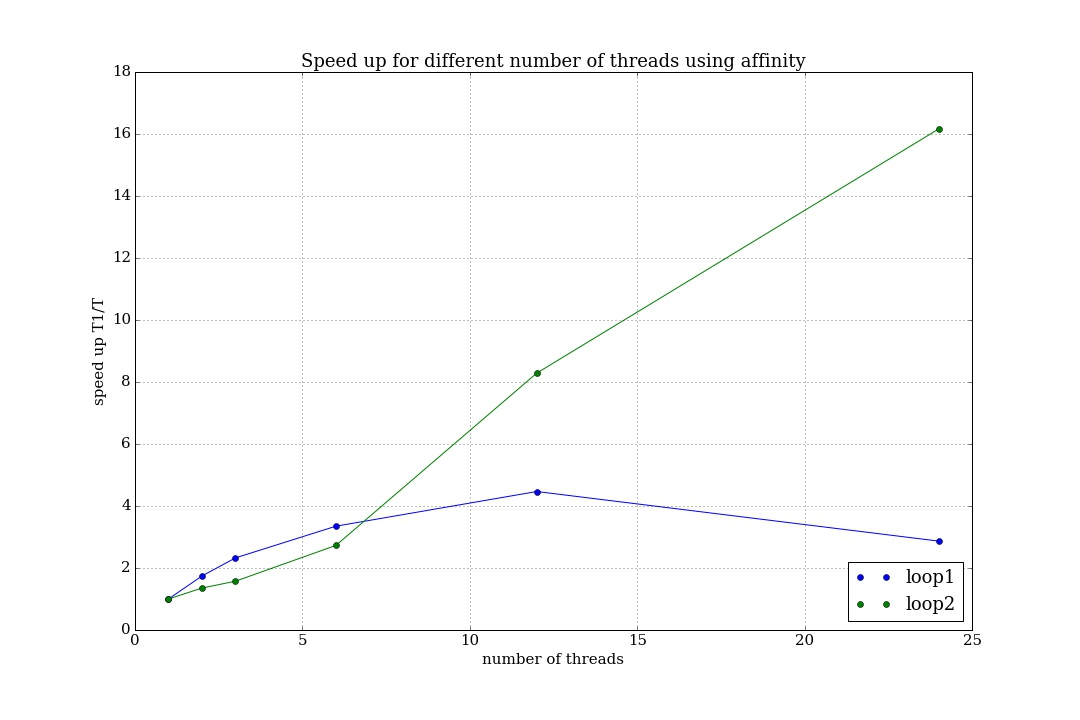
\includegraphics[scale=0.4]{speed_up_af.jpeg}
		\caption{Relative execution time for both function for different number of threads using the new affinity implementation.}\label{upaf}
	\end{figure}

	Figure \ref{upaf} presents the speed up of the affinity using a different number of threads. Again, the values are normalised against the time required by one thread to execute the code. It can be seen that for the more complex function (loop2), the execution time is continuously dropping with more threads used, thus an increase in speed up. For 24 threads, there is a 16x speed up for loop2. This continuous increase in speed up is due to the complexity of the function, as the time required to execute each chunk is much longer than the time it spends looking for the most loaded threads. 
	
	However, for the simpler function, it can be observed an initial speed up, followed by a decrease in speed up. While the execution time using 24 threads is still lower than the execution time using just one thread, this shows how more threads are not beneficial for simpler functions. The behaviour is cause by the overhead time produced as each free thread waits to search for the most loaded thread not compensating for the time it took the thread to execute that new found chunk. 

	\begin{figure}[H]	
		\centering
		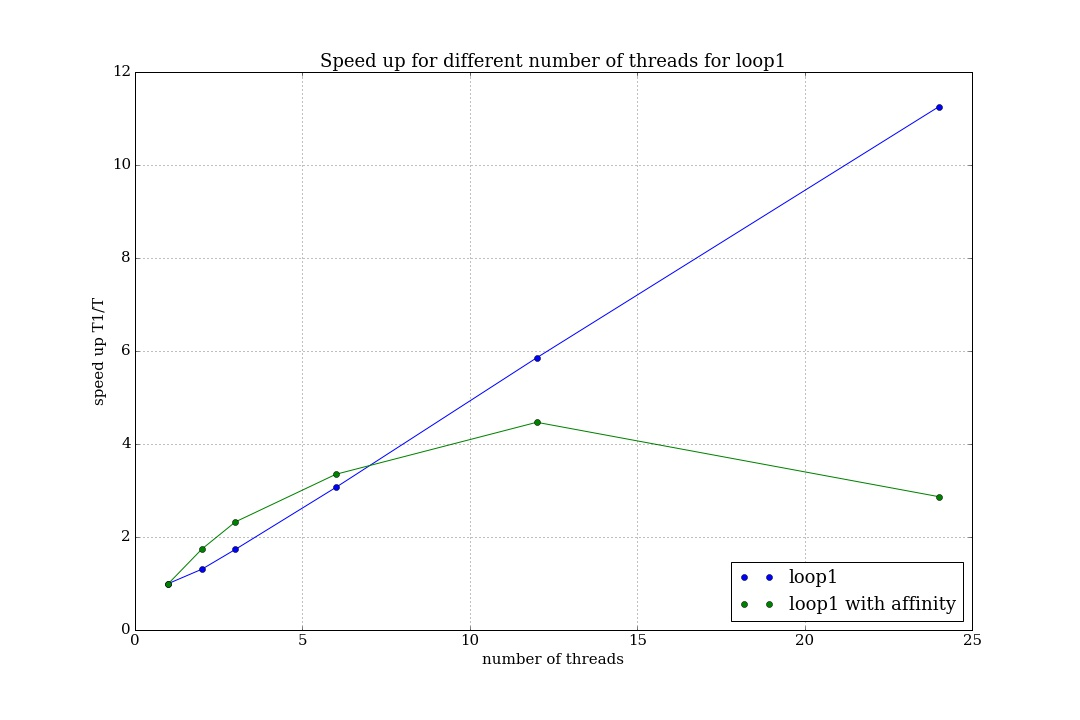
\includegraphics[scale=0.4]{speed_up_l1.jpeg}
		\caption{Relative execution time for loop1 using the simple static and the affinity. }\label{upl1}
	\end{figure}
	
	Figure \ref{upl1} presents the execution speed up for loop1 using the initial determined schedule (static) and the new affinity method. It can be seen clearly that the using affinity scheduling provides a worse execution time, compared with the default scheduling. In addition, if the actual execution times are compared, the static schedule required $0.045269s$, while affinity required $0.191396s$, for the case where just 1 thread was used. This is already a 4.44 times increase in execution time for the affinity schedule. As such, the graph shows that for functions with lower complexity, it is better to use less complex scheduling options.
	
	Figure \ref{upl2} shows the execution speed-up for the the second function, loop2, using the dynamic schedule with chunksize of 4, and the create affinity schedule. From the graph, it can be seen that the dynamic is somewhat more efficient as a speed-up for almost all number of threads used, except for the largest number of threads used. In the last value, it can be seen that affinity just overtakes dynamic in the speed-up factor. However, if the actual execution times are taken into consideration, Figure \ref{upl22}, it can be seen that affinity has a lower execution time for only one thread. In the end, it goes back to being the fastest method. 
	
	Such behaviour can be explained that the dynamic has a better optimisation of overhead for lower numbers of threads. However, if a higher number of threads would be used, affinity would take the lead considerably. In addition, it should be noted that affinity behaves somewhat as the dynamic, as it reduces the chunksize from the initial to a lower one. However, in this case, the dynamic schedule reduces to a chunksize of 4, while affinity reduces to a chunksize of 1. If a default dynamic schedule would be used for comparison (with chunksize of 1, as default), an event better performance comparison could be seen for affinity. 
	
	Function loop2 shows how the affinity schedule can perform similarly to a in built schedule from OpenMP. However, this performance is only observed at more complex functions functions, in which the execution time is quite long.
	
	\begin{figure}[H]	
		\centering
		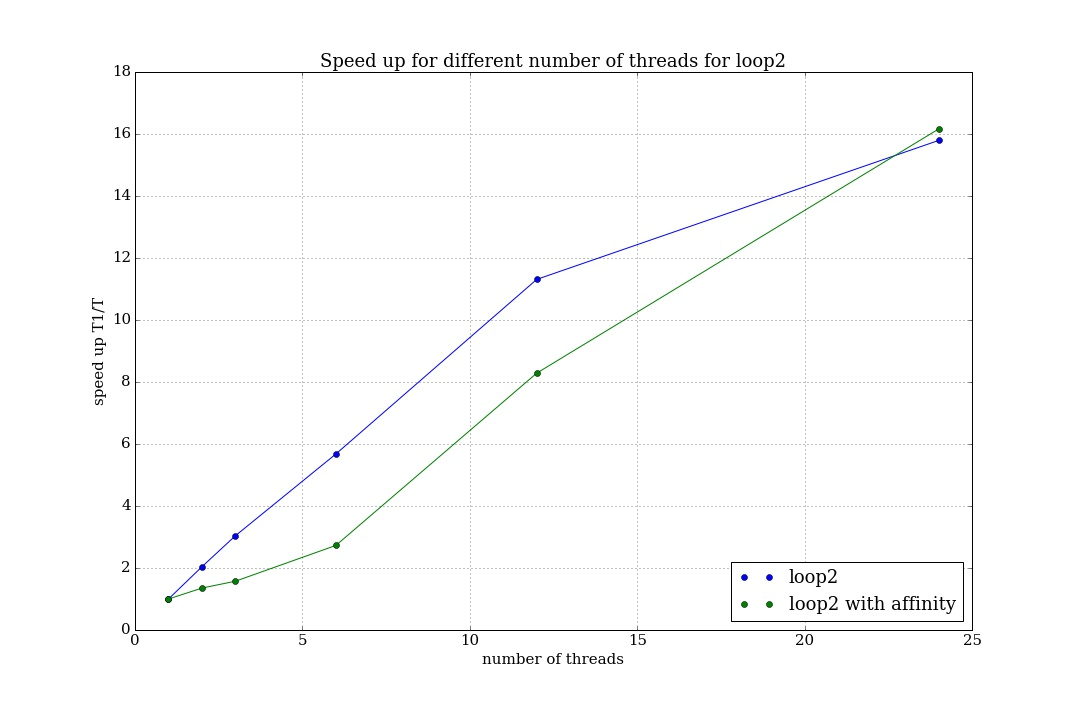
\includegraphics[scale=0.4]{speed_up_l2.jpeg}
		\caption{Relative execution time for both function for different number of threads.}\label{upl2}
	\end{figure}

	\begin{figure}[H]	
		\centering
		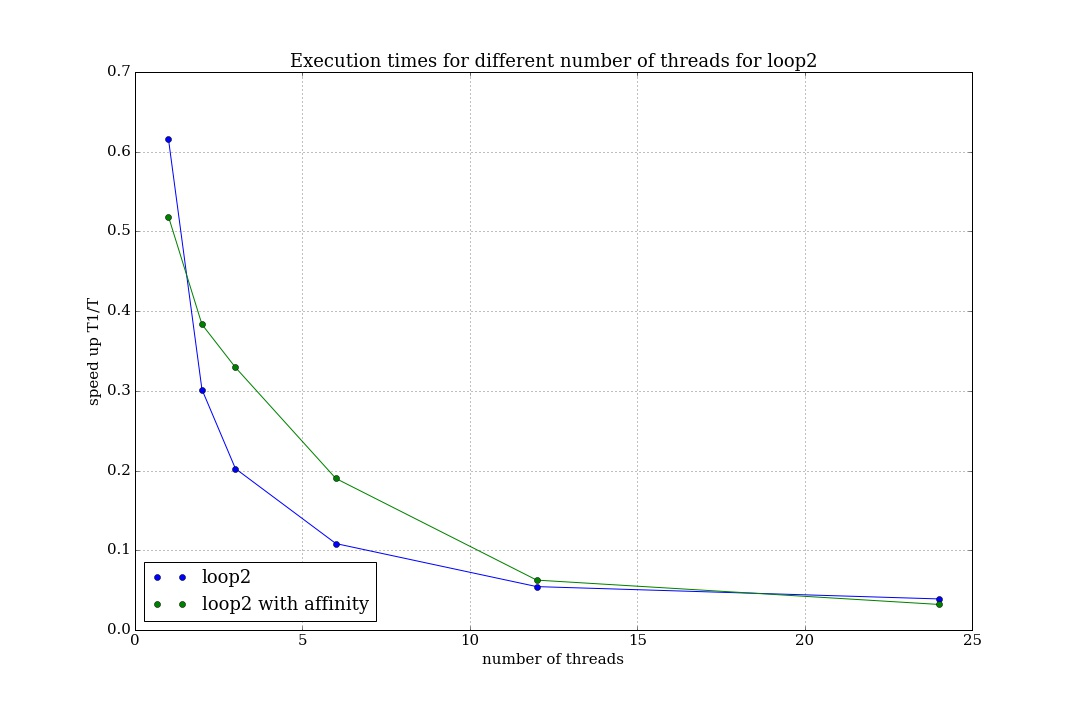
\includegraphics[scale=0.4]{speed_up_l22.jpeg}
		\caption{Execution time for both function for different number of threads.}\label{upl22}
	\end{figure}
	
	
	\section{Conclusion}
	Throughout this exercise, different scheduling methods have been investigated for a relatively simpler function and a more complex function. Firstly, the default schedules for paralellisation were implemented for each function. It was thus concluded that for a function loop1 (the simpler function), a default static schedule gave the best performance, while for the more complex function, the dynamic schedule with a final chunksize of 4 provided the least execution time. These conclusion were drawn while using 6 threads for parallelisation. Secondly, it was then shown the speed up performance when using these schedules with a different number of threads. Loop2 function has shown to have a better speed up than loop1, while both function having a linear speed up profile.
	
	Next, a new schedule method was created an implemented on each function. The affinity schedule provided a considerable speed up for the more complex function, while it generated a relatively small speed up for the simpler function. In addition, the actual execution times were much greater for the simpler function while using affinity compared to the static schedule case. As such, for a simpler function, the static schedule is recommended to be used. 
	
	For the loop2 function, a more complex algorithm, it was shown that the speed-up of the affinity was quite similar to the Dynamic schedule. The effect is due to the fact that executing chunks of iterations in loop2 required more time, thus giving more opportunity for the free threads to search for the busy threads and selecting them, rather than queuing. In addition, it can be possible for the affinity to greatly outperform the dynamic schedule, if additional conditions are imposed and a higher number of threads are used. However, for this function, both methods of scheduling the parallelisation provide good speed-ups in terms of execution times. 
	
\end{document}